\section{Platooning di veicoli}
\fancyhead[RO,LE]{Platooning di veicoli}

Utilizziamo il metodo descritto nell'articolo \cite{ploeg_2014_lp}.


\subsection{Modello matematico del platooning}

\begin{figure}[H]
    \centering
    \captionsetup{justification=centering, margin=2cm}
    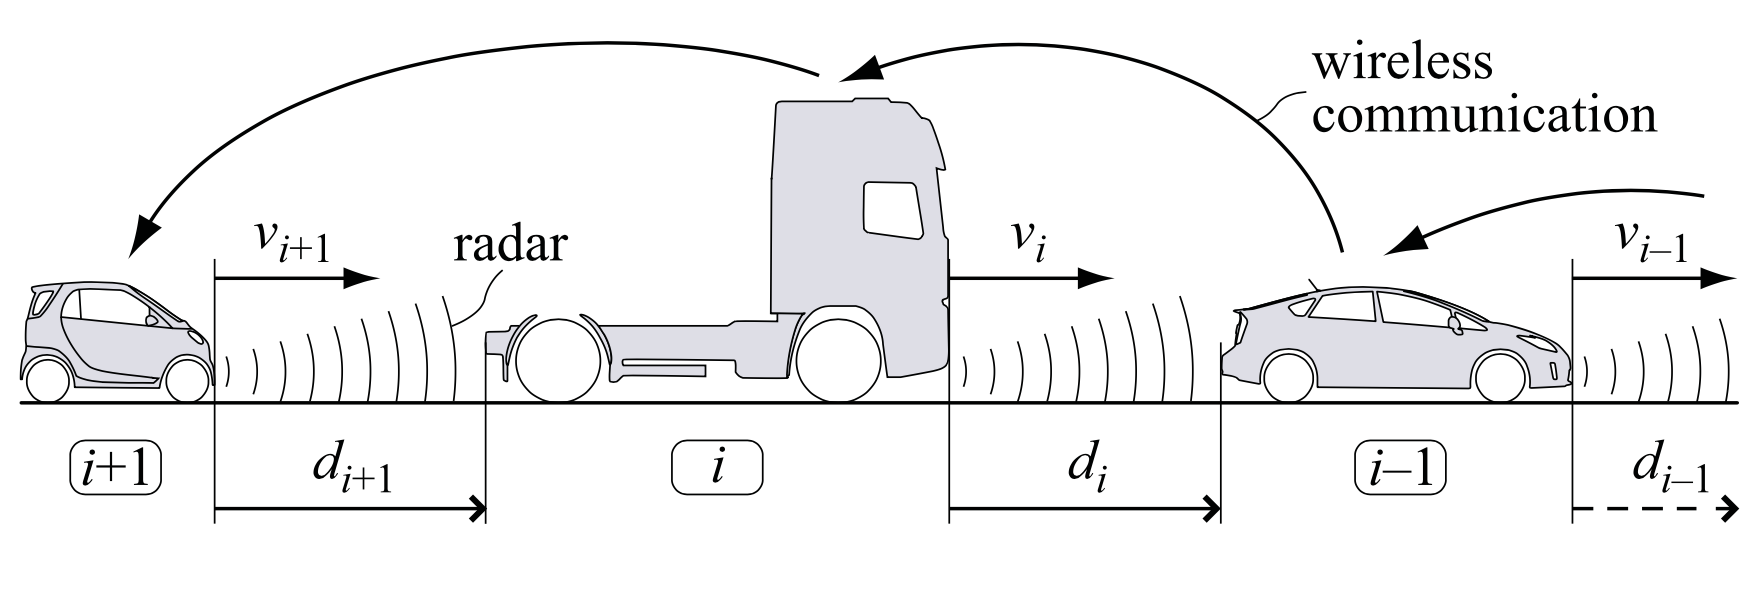
\includegraphics[width=\textwidth]{images/2-theory/PWN-CACC-equipped-vehicle-platoon.png}
    \caption{Platoon di veicoli equipaggiati con CACC}
    \label{fig:cacc-vehicle}
\end{figure}

\newpage
\subsection{Equazioni in forma matriciale}
% Matrici platoon
$\begin{bmatrix}
    \Dot{e}_i \\
    \Dot{v}_i \\
    \Dot{a}_i \\
    \Dot{u}_i
\end{bmatrix}$ = 
$\begin{bmatrix}
    0 & -1 & -h & 0 \\
    0 & 0 & 1 & 0 \\
    0 & 0 & -\frac{1}{\tau} & \frac{1}{\tau} \\
    \frac{k_p}{h} & -\frac{k_d}{h} & -k_d-\frac{k_{dd}(\tau-h)}{h\tau} & -\frac{k_{dd}h+\tau}{h\tau}
\end{bmatrix}$ · 
$\begin{bmatrix}
    e_i \\
    v_i \\
    a_i \\
    u_i
\end{bmatrix}$ +
$\begin{bmatrix}
    0 & 1 & 0 & 0 \\
    0 & 0 & 0 & 0 \\
    0 & 0 & 0 & 0 \\
    0 & \frac{k_d}{h} & \frac{k_{dd}}{h} & \frac{1}{h} \\
\end{bmatrix}$ · 
$\begin{bmatrix}
    e_{i-1} \\
    v_{i-1} \\
    a_{i-1} \\
    u_{i-1}
\end{bmatrix}$
\newline
\newline
Riassunta: $\Dot{x}_i = A_0x_i + A_1x_{i-1}$
con $x_i = (e_i, v_i, a_i, u_i)^t$ che rappresenta il vettore allo stato $i$.

\noindent Svolgiamo il prodotto fra matrici trascurando il fattore $k_{dd}$ che poniamo a $0$ e otteniamo:
\newline

\noindent L'errore: \(\Dot{e}_i = -v_i - ha_i + v_{i-1}\)
\newline

\noindent La velocità: \(\Dot{v}_i = a_i\)
\newline

\noindent L'accelerazione: \(\Dot{a}_i = -\frac{a_i}{\tau} + \frac{u_i}{\tau} = \frac{-a_i+u_i}{\tau}\)
\newline

\noindent Il controllo: \(\Dot{u}_i = \frac{k_p}{h}e_i -\frac{k_d}{h}v_i - k_da_i - \frac{u_i}{h} + \frac{k_d}{h}v_{i-1} + \frac{u_{i-1}}{h} = \frac{k_pe_i - k_dv_i - u_i + k_dv_{i-1} + u_{i-1}}{h} - k_da_i\)

\newpage
\subsection{Campionamento e discretizzazione delle equazioni}

%STAND-ALONE EQUATION EXAMPLE
%\[ x^n + y^n = z^n \]